\begin{appendices}
\chapter{Instruction to execution}
\section{File Structure}
The environment must be installed as the Table~\ref{table:1}. 
It is recommended to use anaconda and set up a virtual environment. GPU server is recommended to use. It will take about 24 hours to train by NVIDIA TITAN V $\times2$.
The file structure is shown as following:
\begin{figure}[ht]
    \centering
    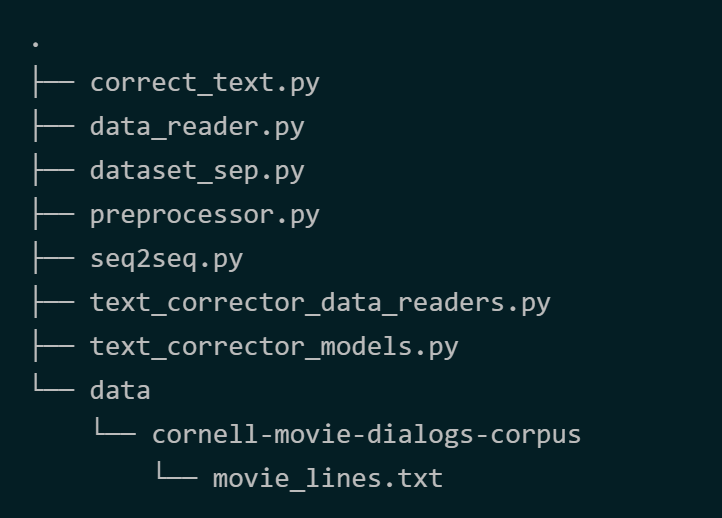
\includegraphics[width=0.8\textwidth]{filest.png}
    \caption{File Structure.}
    \label{fig:11}
\end{figure}
\section{Train and Test}
The following command can be used for training.
\begin{lstlisting}
correct_text.py     --train_path PATH OF TRAINING DATA
                    --val_path PATH OF VALIDATING DATA
                    --config DefaultMovieDialogConfig 
                    --data_reader_type MovieDialogReader
                    --model_path PATH OF SAVED MODEL
\end{lstlisting}
After training, the trained model can be loaded by the following command.
\begin{lstlisting}
model = create_model(sess, True, model_path, config=config)
\end{lstlisting}
To test the trained model, the following command can used.
\begin{lstlisting}
correct_text.py     --test_path PATH OF TESTING DATA
                    --config DefaultMovieDialogConfig 
                    --data_reader_type MovieDialogReader 
                    --model_path /movie_dialog_model
                    --decode
\end{lstlisting}

\end{appendices}